\documentclass[runningheads]{llncs}
%
\usepackage[T1]{fontenc}
% T1 fonts will be used to generate the final print and online PDFs,
% so please use T1 fonts in your manuscript whenever possible.
% Other font encondings may result in incorrect characters.
%
\usepackage{graphicx}
\usepackage{caption}
\usepackage{subcaption}
\usepackage{subfig}
% Used for displaying a sample figure. If possible, figure files should
% be included in EPS format.
%
% If you use the hyperref package, please uncomment the following two lines
% to display URLs in blue roman font according to Springer's eBook style:
%\usepackage{color}
%\renewcommand\UrlFont{\color{blue}\rmfamily}
%
\usepackage[alpha]{mdpn}
\usepackage{tikz}
\usetikzlibrary{positioning,angles,quotes}
\usepackage{algorithm}
\usepackage[noend]{algpseudocode}
\usepackage{program}
\tikzset{%
  every neuron/.style={
    circle,
    draw,
    minimum size=1cm
  },
  neuron missing/.style={
    draw=none, 
    scale=4,
    text height=0.333cm,
    execute at begin node=\color{black}$\vdots$
  },
}
%
\begin{document}
%
\title{Solving Markov Decision Processes using Deep Q-learning}
%
%\titlerunning{Abbreviated paper title}
% If the paper title is too long for the running head, you can set
% an abbreviated paper title here
%
\author{Andrey Antonowycz}
%
\authorrunning{Andrey Antonowycz}
% First names are abbreviated in the running head.
% If there are more than two authors, 'et al.' is used.
%
\institute{University of Twente}
%
\maketitle % typeset the header of the contribution
%
\begin{abstract}
Q-learning is a model-free machine learning algorithm used to determine the optimal action for a given input state. This is achieved by navigating through a model and recording rewards when crossing a transient between two states. The action taken, along with the state it was taken in is recorded and the reward along with possible rewards in the new post-transient state are recorded in an ever-expanding table. The method of optimizing using Q-learning for a given property has proven useful in existing tools \cite{modest} for solving properties in Markov Decision Processes (MDPs). Deep Q-learning is similar in its method of recording, but replaces the process of querying a Q-table with querying a neural network. However, together with other Reinforcement Learning (RL) techniques, it is most often used in domains other than model checking. E.g., finding the optimal action to take given a set of environmental factors and a constant action space. In this paper we are interested in the applicability of using a Deep Q neural network to solve properties in a PRISM model. We will compare different approaches in encoding the action space, and evaluate the accuracy of the resulting model. Multiple methods of encoding the action space are evaluated, including a one-hot encoding and an ordinal encoding. Furthermore, when encoding the action space as either one-hot or ordinal, either a Q-table approach and an input layer approach is utilized. The effects of Double Q-learning as opposed to regular Q-learning are compared, where in Double Q-learning the target and policy network are separated.

\keywords{Model checking \and MDP \and Deep Q-learning.}
\end{abstract}
%
%
%
\newpage
\section{Introduction}

\subsection{Q-learning}

Q-learning is a model-free machine learning algorithm used to determine the optimal action for a given initial state. In model checking the Q-value of the optimal (minimal or maximal, depending on the property to be checked) is the solution to the expected value property. The Q-value is initialized to $0$ for all states, and is updated using the following formula:

\begin{equation}
    Q(s, a) \leftarrow Q(s, a) + \alpha \cdot (r + \gamma \cdot \max_{a'} Q(s', a') - Q(s, a))
\end{equation}

Here $Q(s, a)$ is the Q-value given state $s$ and action $a$. $\alpha$ is the learning rate, which determines how much the Q-value is updated in relation to the reward the model can optimally gain from state $s$. A high learning rate can lead to faster convergence at best, and overshooting at worst. A low learning rate can lead to slower convergence. $\gamma$ is the discount factor, which determines how much the model values rewards which are further away in the future in relation to rewards which are directly reachable. The Q-value given a state-action pair is updated by the difference between the current Q-value and the new Q-value, which is the sum of the reward $r$ and the maximum Q-value of the next state $s'$ and all possible actions $a'$.

During the process of updating the Q-value, the model can either choose to `explore' or `exploit', the former means the model will take a transition which is not optimal, and the latter means the model will take the optimal transition. The exploration rate $\epsilon$ determines the probability of the model to explore. A high exploration rate can lead to a more accurate value, as Q-values of states which are not optimal are also updated and these can influence the Q-value of the optimal transition. A low exploration rate can lead to a faster convergence, as the model will more often take the optimal transition. The exploration rate is generally gradually decreased over time, as the model becomes more accurate. In this paper, the exploration rate is decreased using the following formula:

\begin{equation}
    \epsilon \leftarrow \epsilon \cdot \epsilon_{decay}
\end{equation}

Here $\epsilon_{decay}$ is the decay rate, which determines how much the exploration rate is decreased. To prevent the exploration rate from becoming $0$, a minimum exploration rate $\epsilon_{min}$ is set. The exploration rate is decreased until it reaches this minimum value.

\subsection{Deep Q-learning}

Deep Q-learning is a variant of Q-learning where the Q-table is replaced by a neural network. The input layer is an encoding of the state (or observation) and the output layer is a collection of Q values. The method of optimizing using Q-learning for a given property has proven useful in existing tools \cite{modest}. To test how Deep Q-learning performs, a model checker has been developed that utilizes a neural network to store its Q-values in the form of weights. The expectation is that the network is able to recognize patterns in actions and states to find the Q-value of the initial state (which provides the solution to the property to be evaluated).
\section{Encoding the state-space}

The state-space of an MDP contains values of variables that are in a given range. The values for these variables can be used to define the states' properties.

In Deep Q-learning the state-space represents the input layer of the neural network. Encoding the information representing the state we are currently in and are requesting a set of Q values for is not straight-forward. There are multiple ways of embedding this information in the input layer, each method has its own strengths and weaknesses.

\subsection{One-hot encoding of state variables}

Encoding a variables' values as one-hot neurons is a method to store data for a nominal data point, i.e., there is no ordering applicable between the values of the variable and any such connection made by a neural network in training will likely work counterproductive. An example would be for an internal variable representing the state we are in. Applying one-hot encoding will create a neuron for every value (looking at the possible range of the model variable) and encode its value as either a ``1'' or a ``0''. Encoding the variable this way will prevent ordinal relationships which do not exist in the real model from forming.

Applying one-hot encoding drastically increases the number of input variables in the input layer. This, in turn, increases the size of the neural network (particularly for fully connected layers as every neuron in layer $A$ is then connected to every neuron in layer $B$. The sudden rise in input variables (as every possible permutation of combinations of values for a given variable is now a valid input) can cause a ``big p'' (too many predictors) problem to occur. Here, a predictor is defined as a variables by which the output variable(s) is derived. A ``big p''-problem is characterized by the relation between $p$, the number of predictors and $n$, the number of samples. In order for the network to learn for all its parameters $p$ it is assumed $p \ll n$ such that there is adequate converge for the $p$-dimensional domain. A higher-dimensional input layer is more complex than a lower-dimensional input layer, as a result these higher-dimensional functions are potentially more complicated and will take more time and training data to properly converge (also called the ``curse of dimensionality'').

\subsubsection{Dummy variable encoding}

Furthermore, when one or more of the input neurons can accurately predict the values of another input neuron (multicollinearity), the accuracy of the individual collinear predictor decreases as a result of the coefficients during the optimization process varying with a high degree for a given small change. The odds of measuring the effects of multicollinearity increases when encoding variables of the state-space in a one-hot encoding.

To combat this, we can omit one of the variables' potential value in the one-hot encoding, as it is already implied by the values of the other variable values combinations. E.g., when we have a variable with three different combinations $0, \dots, 3$ we can encode this in one-hot by the following three combinations: $[1, 0, 0]$, $[0, 1, 0]$, $[0, 0, 1]$. To get rid of multicollinearity we can remove one of the variable to convey the same information with fewer neurons: $[1, 0]$, $[0, 1]$, $[0, 0]$. Instead of the sum of all variables being one, there is now the possibility for the sum to be zero and there is no longer a direct correlation between multiple variables in the array.

\subsection{Ordinal encoding of state variables}

Contrary to the discussed method of one-hot encoding a variables to multiple input neurons, where the sum of the values of the individual neurons always equals one, is the alternative method of ordinal encoding. Here the value of the input neuron is represented by the value of the variable directly. The network is able to find patterns and discern between the values of the variable when there is a clear ordinal relationship between its different possible values. When considering the domain of model checking, variables that are valid candidates for an ordinal encoding are counters, clocks of any kind. To discern which variables should be encoded as one-hot or ordinal we can record metadata in the ``JANI'' or ``Modest'' file or perform heuristics, along with a possible manual override in the model checker itself.
\section{Encoding the action-space}
The output layer of the neural network represents the action space, directly corresponding to one or more Q-values. In the most simple cases where the action space is constant (i.e., for every state, the same actions can be taken regardless of any internal variable values) it is common to output a Q-value for every action, resulting in a row of output neurons. I.e., every action has a corresponding output neuron and the neural network only has to be evaluated once in order to output this set of Q-values. Then, the $argmax$ the row of Q-values is the optimal action.
Contrary to regular Q-learning where we are able to expand an ever-increasing Q-table with state-action pairs, the size of the neural network (including the size of the output layer) has to be predefined before the training process. Deep Q-learning is often applied to environments with a constant action space, where its dimensionality is independent of the input state. This is common for games or well-known optimization problems like ``CartPole'', where all transitions (e.g., move left, move right) are always enabled. In the domain of model checking this is untrue in most cases, the enabled transitions vary for the state of the automaton and the values of the state variables which determine the guard values. An alternate method of encoding the action space is therefore to disregard the convention of multiple Q-values as output, and to encode the complete state-action pair as the input layer. The output of the neural network then becomes a single Q-value. In the following section the difficulties in encoding the action-space and the advantages and disadvantages of various methods of encoding the action space are discussed.

\subsubsection{Parallel composition}
A model can contain multiple parallel automatons, each automaton is in a certain state and has a certain value for the variables allocated in its namespace. The scheduler can then choose an action for any of the automatons, and depending on the values of its variables and the predefined synchronization vectors, multiple automatons can synchronize. One possible solution for the problem of action-space encoding is the record the largest number of possible commands an automaton can make for any given state it can be in and set the number of output neurons equal to that number. For any given state at any given time we then order the possible commands in a constant manner. However, for a model containing more than one automaton, it is ambiguous to which action the output neurons correspond to; i.e., which scheduler do we choose? Creating a different neural network for the different automatons is not a solution either because we are interested in the interplay between the behaviors and variables in each automaton.

\subsubsection{Process synchronization}
In an MDP with multiple independent automatons there exists the possibility for multiple transitions two synchronize. When this occurs all automatons are advanced to the future state in accordance with their appropriate $(s, t, s')$ tuple. Whether and when a transition of a given automaton can synchronize with the transitions of another automaton depends on the synchronization vectors. Given a synchronization vector $(\alpha, -, \beta, \tau)$, automaton $0$ is able to synchronize transition label $\alpha$ with automaton $2$ with transition label $\beta$ and automaton $3$ with transition label $\tau$. However, given one of said automatons, there can be no or multiple transitions enabled with the transition label required for synchronization. Encoding all possible permutations in the action space as a single action each poses the problem of a possible action-space explosion. When encoding the different possible options all falling under the same synchronization vector as the same action will not yield accurate results as action with the same label yet different futures (can) yield different rewards.

\subsection{Solutions}
When considering a model encoded in the JANI \cite{jani} or Modest \cite{modest} format, the label given to an action has no particular meaning other than human-readability and synchronization. The transition label itself does not provide ample distinction as the model checker allows for an overlap in the transition labels. For example, for a given state there can be multiple outgoing transitions with label $a$, and this label can occur in multiple different automatons. There is no connection between the transitions all identifying as $a$, and training the model in a way that does not discern between these transitions can yield incorrect results. For regular Q-learning this does not pose a problem as we can simply record the command for this specific state in the Q-table, there is no definition collision between this action for this state with similar actions in other states. Furthermore, for a given transition there can be multiple enabled guards in case the guard conditions are overlapping. In this case there are multiple transitions applicable for a given transition label in a state for a given set of variables that are evaluated against a set of guard expressions. Because of this discrepancy between regular Q-learning and Deep Q-learning the output layer should be encoded to account for the varying action space. To achieve this, one can consider multiple potential solutions.

\subsubsection{One-to-one mapping of neurons and commands}
If we consider every command (specifically discerning between overlapping guard expressions like $k \ge 0$ and $k = 0$ which collide at $k = 0$) we end up with a unique output neuron for every possible action the model can take. This means we end up with an action space that grows exponentially with the number of states, as every action in every state adds $n$ actions to the output layer. When considering fully connected layers between the output neurons and the rest of the network this quickly becomes unfeasible when optimizing for large models, and a regular Q-table would be more efficient and more accurate. Additionally we need to consider the problem of choosing a correct action; the output layer contains the predicted Q-values for every action. This includes Q-values for actions which are non-applicable in the state of interest. This is not the case for models with a constant action space and in regular Q-learning, in these cases every Q-value and matching action in the output layer or Q-table can be considered at all times. If we only select a very small subset of the output layers' data, the model will not learn what to do with most neurons in most cases as it's only being tested against some of its outputs at one particular time. There may even be output neurons which are (nearly) never used or validated against because of the chosen scheduler.

\subsubsection{Flattened model representation}
When solving for models with multiple automatons, synchronized transitions can pose a problem. In particular, when a transition in one automaton is synchronized with a transition in another automaton, the action space is not only dependent on the state of the automaton, but also on the state of the other automaton. Furthermore, a synchronized transition can span any number of automatons in the model, drastically increasing the complexity of accounting for this behavior in a Deep Q-learning model. Figure \ref*{fig:mdp_parallel} shows an example where two processes $P$ and $Q$ can only take transition $a$ simulatiniously if and only if $P$ is in state $p_1$ and $Q$ is in $q_1$.

\begin{figure}
  \centering
  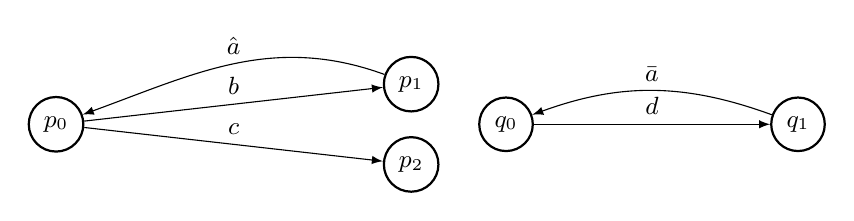
\begin{tikzpicture}[auto,node distance=8mm,>=latex,font=\small]
      \tikzstyle{round}=[thick,draw=black,circle]
      
      \node[round] (p0) {$p_0$};
      \node[round,above right=0mm and 40mm of p0] (p1) {$p_1$};
      \node[round,below right=0mm and 40mm of p0] (p2) {$p_2$};
      
      \draw[->] (p0) -- node[above] {$b$} (p1);
      \draw[->] (p1) [out=160,in=20] to node[above] {$\hat{a}$} (p0);
      \draw[->] (p0) -- node[above] {$c$} (p2);

      \node[round, right=0mm and 50mm of p0] (q0) {$q_0$};
      \node[round, right=0mm and 30mm of q0] (q1) {$q_1$};
      
      \draw[->] (q0) -- node[above] {$d$} (q1);
      \draw[->] (q1) [out=160,in=20] to node[above] {$\bar{a}$} (q0);
  \end{tikzpicture}
  \caption{MDP with two processes $P$ and $Q$, for which transitions $\hat{a}$ and $\bar{a}$ are synchronized. Transition $a$ can be taken in $P$ and transition $a$ can be taken in $Q$ at the same time if both models are in state $p_1$ and $q_1$ respectively.}
  \label{fig:mdp_parallel}
\end{figure}

A possible solution to the issues arising from synchronization is to consider the flattened MDP model instead. Here all the behavior of the individual automatons is expressed as a single main automaton. This has the advantage of not having to account for the different possible transitions required for a transition to synchronize. However, this approach has several caveats. For one, the model that results from the flattening is more complex than the original model. Ideally, there is a method of encoding the state-action pair and its subsequent Q-value in such a way that a non-flattened model would suffice. The behavior of a simple clock, for example, which dictates whether a transition can be taken in another automaton is now embedded in a more complex main automaton. Flattening the model in figure \ref{fig:mdp_parallel} results in the model in figure \ref{fig:mdp_flattened}.

\begin{figure}
  \centering
  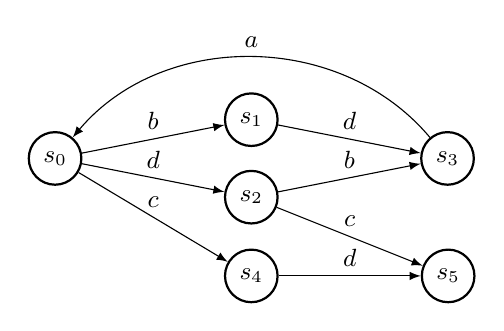
\begin{tikzpicture}[auto,node distance=8mm,>=latex,font=\small]
      \tikzstyle{round}=[thick,draw=black,circle]

      \node[round] (s0) {$s_0$};
      \node[round,above right=0mm and 20mm of s0] (s1) {$s_1$};
      \node[round,below right=0mm and 20mm of s0] (s2) {$s_2$};
      \node[round,above right=0mm and 20mm of s2] (s3) {$s_3$};

      \node[round,below right=10mm and 20mm of s0] (s4) {$s_4$};
      \node[round,below right=10mm and 45mm of s0] (s5) {$s_5$};

      \draw[->] (s0) -- node[above] {$b$} (s1);
      \draw[->] (s0) -- node[above] {$d$} (s2);
      \draw[->] (s1) -- node[above] {$d$} (s3);
      \draw[->] (s2) -- node[above] {$b$} (s3);
      \draw[->] (s3) [out=130,in=50] to node[above] {$a$} (s0);
      \draw[->] (s0) -- node[above] {$c$} (s4);
      \draw[->] (s2) -- node[above] {$c$} (s5);
      \draw[->] (s4) -- node[above] {$d$} (s5);
  \end{tikzpicture}
  \caption{Flattened model representation of the model illustrated in figure \ref{fig:mdp_parallel}. This model contains just one automaton, and the behavior of the original model is expressed in this single automaton.}
  \label{fig:mdp_flattened}
\end{figure}

Flattening the model results in a single automaton that is strongly bisimilar to the behavior of the separate original automatons. The main advantage of this approach is the negation of the synchronization between the individual automatons, and the simpler encoding of the action space it enables. It also reduces the number of overlapping actions caused by synchronization. For example, if action $a$ in automaton $0$ and action $b$ in automaton $1$ are included in the same synchronization vector, choosing either action will have the same effect on the network; automaton $0$ will take transition $a$ and automaton $1$ will take transition $b$. In the flattened model it is no longer ambiguous which automaton should be addressed, and there is no overlap in actions between different network components.

If we now consider the maximum number of actions in any location, which can be easily extracted from the flattened model, to be the size of the action space we have a significantly smaller array of options.

\begin{figure}[h]
    \centering
    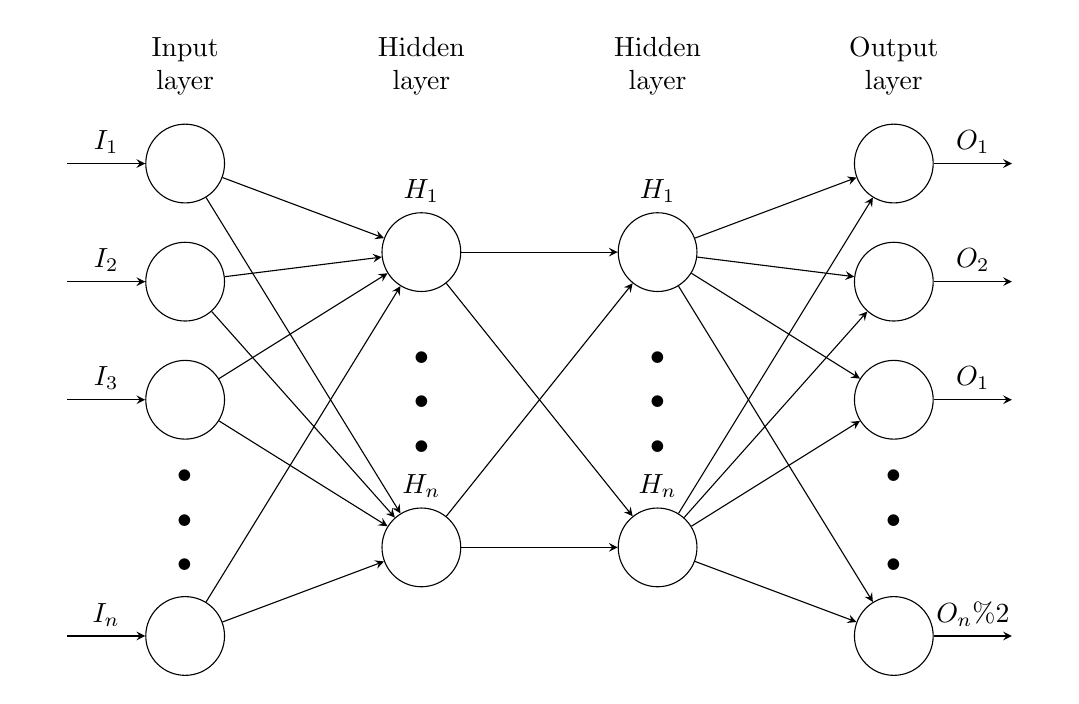
\begin{tikzpicture}[x=1.5cm, y=1.5cm, >=stealth]
    
    \foreach \m/\l [count=\y] in {1,2,3,missing,4}
      \node [every neuron/.try, neuron \m/.try] (input-\m) at (0,2.5-\y) {};
    
    \foreach \m [count=\y] in {1,missing,2}
      \node [every neuron/.try, neuron \m/.try ] (hidden0-\m) at (2,2-\y*1.25) {};
    
    \foreach \m [count=\y] in {1,missing,2}
      \node [every neuron/.try, neuron \m/.try ] (hidden1-\m) at (4,2-\y*1.25) {};
    
    \foreach \m [count=\y] in {1,2,3,missing,4}
      \node [every neuron/.try, neuron \m/.try ] (output-\m) at (6,2.5-\y) {};
    
    \foreach \l [count=\i] in {1,2,3,n}
      \draw [<-] (input-\i) -- ++(-1,0)
        node [above, midway] {$I_\l$};
    
    \foreach \l [count=\i] in {1,n}
      \node [above] at (hidden0-\i.north) {$H_\l$};
    
    \foreach \l [count=\i] in {1,n}
      \node [above] at (hidden1-\i.north) {$H_\l$};
    
    \foreach \l [count=\i] in {1,2,1,n \% 2}
      \draw [->] (output-\i) -- ++(1,0)
        node [above, midway] {$O_\l$};
    
    \foreach \i in {1,...,4}
      \foreach \j in {1,...,2}
        \draw [->] (input-\i) -- (hidden0-\j);
    
    \foreach \i in {1,...,2}
      \foreach \j in {1,...,2}
        \draw [->] (hidden0-\i) -- (hidden1-\j);
    
    \foreach \i in {1,...,2}
      \foreach \j in {1,...,4}
        \draw [->] (hidden1-\i) -- (output-\j);
    
    \foreach \l [count=\x from 0] in {Input, Hidden, Hidden, Output}
      \node [align=center, above] at (\x*2,2) {\l \\ layer};
    
    \end{tikzpicture}
    \caption{Graphical representation of a neural network with $n$ output neurons, where the associated action $a$ for a location with $2$ actions corresponds to output neurons where $n \% 2 = a$.}
    \label{fig:nn_mod}
\end{figure}

We can then encode the actions in such a way that there is not a possibility for an ``invalid transition'', i.e. an action which is not enabled in the current state, to be taken at any moment. This is achieved by computing the modulo of the output neuron index with respect to the number of enabled actions in the current state (e.g., figure \ref{fig:nn_mod}). The resulting action index will always have a corresponding enabled action. However, there is a scalar of issues that arises from this approach. The first and foremost issue is caused by guards and their effect on the enabled transitions. If we consider an MDP where the number of enabled actions depends on the value of a state variable (e.g., figure \ref{fig:mdp_enabled_action_count}) we encounter a problem if we encode and decode the action based on the number of enabled actions. In this figure action $a$ is either not listed as an enabled action when $k = 0$, or listed as an enabled action after the network has traversed to $s_1$ via action $b$ and back to $s_0$ via action $\tau$ at least once, resulting in the guard $k > 0$ being satisfied.

\begin{figure}
    \centering
    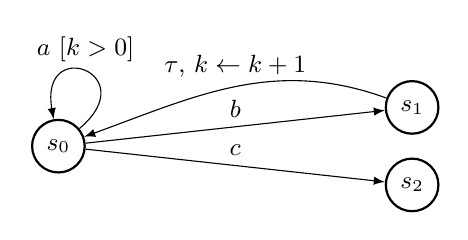
\begin{tikzpicture}[auto,node distance=8mm,>=latex,font=\small]
        \tikzstyle{round}=[thick,draw=black,circle]
        
        \node[round] (s0) {$s_0$};
        \node[round,above right=0mm and 40mm of s0] (s1) {$s_1$};
        \node[round,below right=0mm and 40mm of s0] (s2) {$s_2$};
        
        \draw[->] (s0) -- node[above] {$b$} (s1);
        \draw[->] (s1) [out=160,in=20] to node[above] {$\tau$, $k \leftarrow k + 1$} (s0);
        \draw[->] (s0) -- node[above] {$c$} (s2);
        \draw[->] (s0) [out=40,in=100,loop] to node[above] {$a$ [$k > 0$]} (s0);
    \end{tikzpicture}
    \caption{MDP for which the action space size is $2$ for $k = 0$ and $3$ for the guard $k > 0$, this poses a challenge to encoding the action space in a neural network as action $b$ could potentially be mapped to either output neuron $1$ or output neuron $2$, depending on the value of $k$.}
    \label{fig:mdp_enabled_action_count}
\end{figure}

\subsubsection{Single Q-value action-space}

If we instead flip the convention of outputting a Q-table after entering the current state as the input layer, and instead output a single Q-value given an observation and action we get a neural network more akin to the mathematical representation of Q-learning. In the mathematical model one considers state-action pairs to be the \emph{key} in the Q-table, and the Q-value to be the \emph{value}. This means the action space needs to be \emph{encoded} in the input layer and therefore does not need to be \emph{decoded} in the output layer.

Having only one output neuron solves several issues considered and touched upon in the sections before. Due to the fact that we are not selecting actions from a table anymore, the possibility of selecting a Q-value belonging to an action not in the action space of the current state is not applicable anymore. Any information we feed into the network (given it is valid information), returns a singular Q-value.

Because the action needs to be encoded in the input layer, new problems arise. For one, the number of input neurons is increased, and as a result the network may be overstimulated in its process to find the correct weights in its optimization efforts. There are several methods of encoding the action space into the input layer. The most straightforward method is to use a similar approach to what was done in decoding the output layer; to consider the enabled actions in a given state and encode the index of this action (either ordinal or one-hot) as the input neuron. This solution worked well for the output layer encoding because we are not in control of what the network outputs, however we \emph{are} in control of what we feed into the network.

This opens the possibility of feeding the raw transition data directly into the network. These are the transition tuples the network in the Modest Python export considers, in which a transition number always corresponds to a single transition for every separate automaton. The behavior of all automatons is encoded in any transition tuple, and therefore process synchronization can be expressed as well. Given this tuple of transitions is gained by querying the network, the tuple is always valid and its transitions are therefore enabled.

\begin{figure}[h]
    \centering
    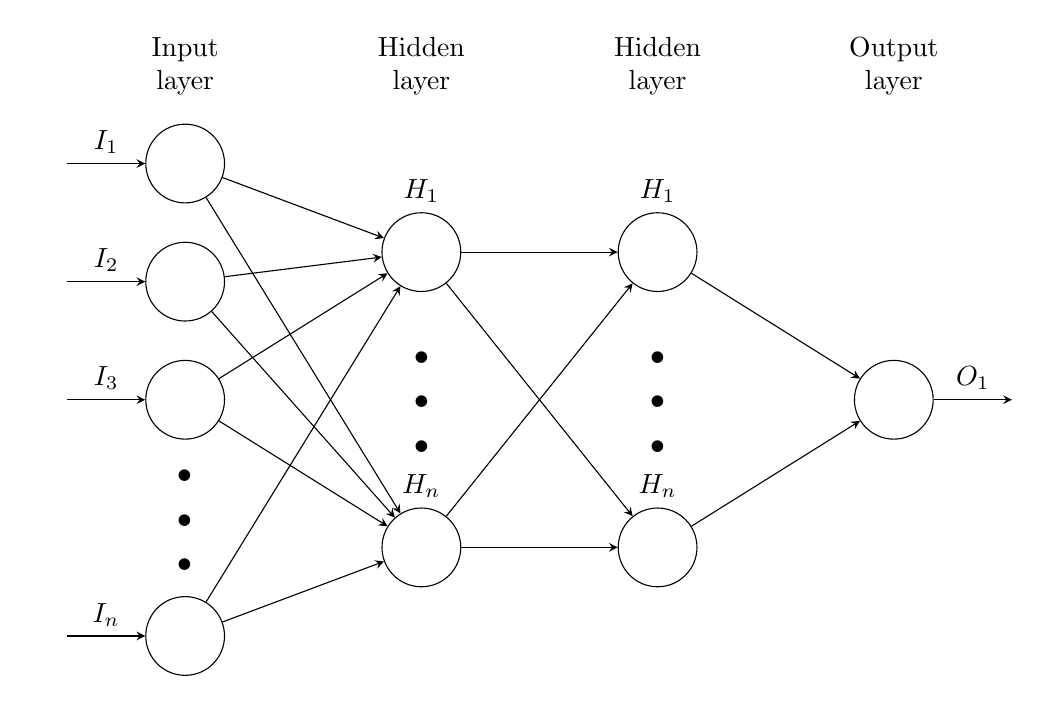
\begin{tikzpicture}[x=1.5cm, y=1.5cm, >=stealth]
    
    \foreach \m/\l [count=\y] in {1,2,3,missing,4}
      \node [every neuron/.try, neuron \m/.try] (input-\m) at (0,2.5-\y) {};
    
    \foreach \m [count=\y] in {1,missing,2}
      \node [every neuron/.try, neuron \m/.try ] (hidden0-\m) at (2,2-\y*1.25) {};
    
    \foreach \m [count=\y] in {1,missing,2}
      \node [every neuron/.try, neuron \m/.try ] (hidden1-\m) at (4,2-\y*1.25) {};
    
    \foreach \m [count=\y] in {1}
      \node [every neuron/.try, neuron \m/.try ] (output-\m) at (6,0.5-\y) {};
    
    \foreach \l [count=\i] in {1,2,3,n}
      \draw [<-] (input-\i) -- ++(-1,0)
        node [above, midway] {$I_\l$};
    
    \foreach \l [count=\i] in {1,n}
      \node [above] at (hidden0-\i.north) {$H_\l$};
    
    \foreach \l [count=\i] in {1,n}
      \node [above] at (hidden1-\i.north) {$H_\l$};
    
    \foreach \l [count=\i] in {1}
      \draw [->] (output-\i) -- ++(1,0)
        node [above, midway] {$O_\l$};
    
    \foreach \i in {1,...,4}
      \foreach \j in {1,...,2}
        \draw [->] (input-\i) -- (hidden0-\j);
    
    \foreach \i in {1,...,2}
      \foreach \j in {1,...,2}
        \draw [->] (hidden0-\i) -- (hidden1-\j);
    
    \foreach \i in {1,...,2}
      \foreach \j in {1,...,1}
        \draw [->] (hidden1-\i) -- (output-\j);
    
    \foreach \l [count=\x from 0] in {Input, Hidden, Hidden, Output}
      \node [align=center, above] at (\x*2,2) {\l \\ layer};
    
    \end{tikzpicture}
    \caption{Graphical representation of a neural network with $1$ output neuron, where the both the state and action is encoded in the input layer.}
    \label{fig:nn_single_q}
\end{figure}
\newpage
\section{Methodology}

\subsection{Batch-learning and experience replay}

When optimizing the neural network for a given (set of) transition(s), there are a multitude of viable approaches. The most straightforward method is to navigate the network for one or more transitions and to optimize based on the loss of the batch of size one or greater. Given a batch of transitions we can compute the average loss using the algorithm in algorithm \ref{algorithm:loss}.

Noteworthy to mention is that only the transition tuples are stored, not the subsequent Q-values, this means that for an observation we store the tuple $(s, a, s', as', r, g, d)$ where $s$ is the initial state, $a$ the action taken from said initial state, $s'$ the state we end up in after taking action $a$ from state $s$ and $as'$ the set of enabled actions in state $s'$. $r$ is the reward that is received from traversing the transient. Additionally, metadata is stored to assign zero Q-values to the appropriate states ($g$ := $s$ is a goal state, $d$ := $s$ is a deadlock state). The Q-values are gathered from the policy- and target network (represented by the same network when not using double Deep Q learning) every iteration and thus consider the Q-values as a result of the updated network weights.

When applying algorithm \ref{algorithm:loss} for any number of transitions it is key to consider applying learning using experience replay. Here, instead of learning solely based off of the latest $x$ transitions we store said transitions in a replay buffer of a predefined maximum size and sample $x$ transitions randomly. If the replay buffer is full, its values are shifted and the oldest values are ejected. What is achieved is a more stable optimization methodology due to the last number of steps not overshadowing the policy updates. This way, earlier transitions encountered are still relevant in the learning process. A larger batch size yields a more varied set of learning data, however the computations will take longer to finish.

\begin{algorithm}
    \caption{Pseudo-code for calculating the loss of a batch of transitions using MSE (mean squared error) given a batch size ($N$) and a batch of transitions characterized by the variables $g$ ($s$ is a goal state), $d$ ($s$ is a deadlock state), $s'$ (the state as a product of the state-action pair transition), $as'$ (the enabled actions in $s'$), $s$ (the state part of the state-action pair transition) and $a$ (the action part of the state-action pair transition), $r$ is the reward from traversing from $s$ to $s'$.}
    \label{algorithm:loss}
    \begin{program}
    \BEGIN \\ %
    Q' := |zeros|(N)
    mask := \lnot g \land \lnot d
    \FOR i := 0 \TO N \STEP 1 \DO
    condition := |mask|[i]
    state := |s'|[i]
    actions := |as'|[i]
    \IF condition; \DO |Q'|[i] := |optimal|(|target_net|(|cat|(state, actions))) \OD \OD \\ \OD
    Q' := (\gamma Q') + r
    Q := |policy_net|(|cat|(s, a))
    loss := |MSE|(Q, Q')
    \END
    \end{program}
\end{algorithm}

\subsection{Double Deep Q-learning}

In Deep Q-learning the value of the Q-values are correlating to one another due to the expected Q-value for state $s$ being defined as $r + \gamma argmax(s', a')$. In cases where there are no deadlock or goal states reached this can cause a positive self-loop where the Q-values explode. There is a common method of reducing the correlation between the expectation and target by sampling the Q-values from different neural networks. The expected Q-values are samples from the target network and the current Q-values are sampled from the policy network. The policy network is then optimized by applying back-propagation on the loss.

\subsubsection{Hard versus soft weight updates}

When using a separate target and policy network in Deep Q-learning it is necessary to (at some point) propagate the weights we acquired using the optimization in the policy network to the target network. Otherwise the expected Q-values that are compared against the live Q-values of the policy network will remain the Q-values as a result of the initial randomized weight initialization. There are two prominent methods of transferring the weights of the policy network to the target network: hard and soft weight updates. When applying hard updating of the weights there is a set number of transitions or optimization steps before the weights are copied over from the policy network to the target network in its entirety. When applying soft weight updating we consider a constant $0 < \tau < 1$, and after every optimization step we update the weights of the target network according to the equation \ref{eq:soft_weight_update} where $\theta'$ is a weight in the target network and $\theta$ is a weight in the policy network.

\begin{equation}\label{eq:soft_weight_update}
    \theta\sp{\prime} \gets \tau \theta + (1 - \tau) \theta\sp{\prime}
\end{equation}

\subsection{MDPs}

Due to the nature of a neural network and its `black box' properties, it was chosen to start with overly simplified models and gradually increase their complexity over time. There are several MDPs chosen to fulfill this role. In this section all MDPs are introduced along with appropriate solutions.

\subsubsection{Single-transition MDP}

The most simple and straight-forward MDP that can be constructed in the domain of reward property expressions is a model with two distinct states $s_0$ and $s_1$ where the transition $(s_0, \tau, s_1)$ yields a certain reward. This model is trivial to solve for most if not all model checkers, but serves as a starting point for the Deep Q-learning model checking experimentation. I.e., if the implemented network is unable to solve this simplest network, there is an inherent error in its implementation and its structure and optimization process needs to be re-established. Its solution is computed to be $8$:
\begin{verbatim}
+ Property R1
  Value:  8
  Bounds: [8, 8]
\end{verbatim}

\begin{figure}[H]
    \centering
    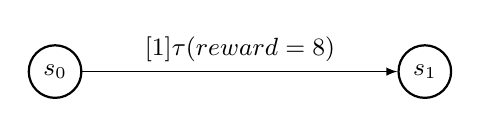
\begin{tikzpicture}[auto,node distance=8mm,>=latex,font=\small]
        \tikzstyle{round}=[thick,draw=black,circle]
        
        \node[round] (s0) {$s_0$};
        \node[round,right=40mm of s0] (s1) {$s_1$};
        
        \draw[->] (s0) -- node[above] {$[1] \tau (reward = 8)$} (s1);
    \end{tikzpicture}
    \caption{MDP with a single transition between two states.}
    \label{fig:single-transition-mdp}
\end{figure}

\subsubsection{Success-fail MDP}

A slightly more complex yet still trivially solvable MDP is one where we omit non-determinism and consider a single transition where there is a $0.5$ chance of reaching $success$ and a $0.5$ chance of reaching $fail$. The property we are checking for then becomes the expected reward in either of the goal states $success$ or $fail$. Its solution is computed to be $4$:
\begin{verbatim}
+ Property R1
  Value:  4
  Bounds: [4, 4]
\end{verbatim}

\begin{figure}[H]
    \centering
    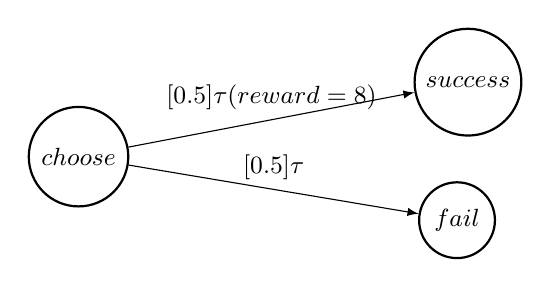
\begin{tikzpicture}[auto,node distance=8mm,>=latex,font=\small]
        \tikzstyle{round}=[thick,draw=black,circle]
        
        \node[round] (choose) {$choose$};
        \node[round,above right=0mm and 40mm of choose] (success) {$success$};
        \node[round,below right=0mm and 40mm of choose] (fail) {$fail$};
        
        \draw[->] (choose) -- node[above] {$[0.5] \tau (reward = 8)$} (success);
        \draw[->] (choose) -- node[above] {$[0.5] \tau$} (fail);
    \end{tikzpicture}
    \caption{Modest MDP with a single transition awarding either a reward or no reward.}
    \label{fig:success-fail-mdp}
\end{figure}

\subsubsection{Risk-safe MDP}

Finally, we introduce a choice between two transitions in the initial state and consider two different properties: the maximum and minimum expected reward. The previously introduced model is modified to include a choice between $risk$ and $safe$. If we choose risk there is a $0.5$ chance of reaching success with a reward of $8$, and if we choose $safe$ there is a $0.9$ chance of reaching success with a reward of $2$. Here we find the maximum and minimum expected rewards to be $4$ and $1.8$ respectively:
\begin{verbatim}
+ Property R1
  Value:  4
  Bounds: [4, 4]
+ Property R2
  Value:  1.8
  Bounds: [1.8, 1.8]
\end{verbatim}

\begin{figure}[H]
    \centering
    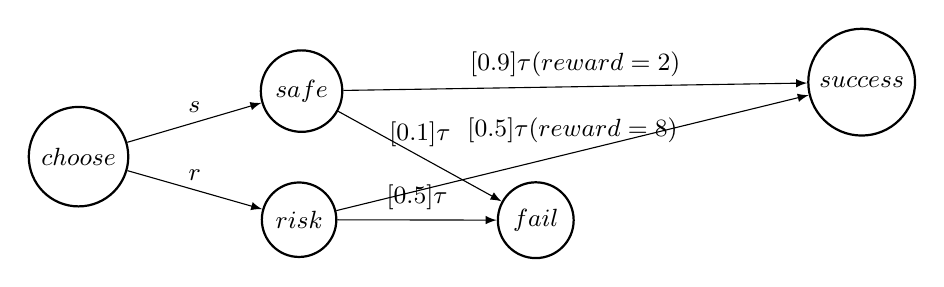
\begin{tikzpicture}[auto,node distance=8mm,>=latex,font=\small]
        \tikzstyle{round}=[thick,draw=black,circle]
        
        \node[round] (choose) {$choose$};
        \node[round,above right=0mm and 20mm of choose] (safe) {$safe$};
        \node[round,below right=0mm and 20mm of choose] (risk) {$risk$};
        \node[round,above right=0mm and 90mm of choose] (success) {$success$};
        \node[round,below right=0mm and 50mm of choose] (fail) {$fail$};
        
        \draw[->] (choose) -- node[above] {$s$} (safe);
        \draw[->] (choose) -- node[above] {$r$} (risk);
        \draw[->] (safe) -- node[above] {$[0.9] \tau (reward = 2)$} (success);
        \draw[->] (safe) -- node[above] {$[0.1] \tau$} (fail);
        \draw[->] (risk) -- node[above] {$[0.5] \tau (reward = 8)$} (success);
        \draw[->] (risk) -- node[above] {$[0.5] \tau$} (fail);
    \end{tikzpicture}
    \caption{Modest MDP with a single choice in the first state between $s$ and $r$, which can take two different paths to success. Either via $safe$ or via $risk$, awarding a reward of $2$ and $8$ respectively. The chance to reach the $fail$ state is greater in $risk$ than it is in $safe$.}
    \label{fig:safe-risk-mdp}
\end{figure}

\subsection{QComp models}

A set of QComp models were chosen to test the Deep Q-learning model checking approach. The models were chosen based on their complexity and the number of states and transitions, as well as the prescence of an \emph{E-}type (expected value type) property. The models are as follows:

\subsubsection{Energy-aware Job Scheduling}

The first QComp model used to test Deep Q-learning is the Energy-aware Job Scheduling MDP \cite{eajs}. In this model, $N$ processes (2 or 4 in the case of this paper) are required to perform tasks given a deadline. The processes request to enter a `critical section' in order to perform their tasks, and consume a certain amount of energy depending whether or not they entered the `critical section' or not. It is possible for the process to exceed its deadline. The property $ExpUtil$ signifies the expected utility gained from the processes, i.e., the number of tasks finished without exceeding their deadline. The property $ExpUtil$ is computed to be $4.028$ for $N = 2$, $energy\_capacity = 100$ and $B = 5$:

\begin{verbatim}
  + Property ExpUtil
    Value:  4.028
    Bounds: [4.028, 4.028]
\end{verbatim}

The property $ExpUtil$ is computed to be $8.0176$ for $N = 2$, $energy\_capacity = 200$ and $B = 9$:

\begin{verbatim}
  + Property ExpUtil
    Value:  8.0176
    Bounds: [8.0176, 8.0176]
\end{verbatim}

\subsubsection{Randomized Consensus Protocol}

The second QComp model used to test Deep Q-learning is the Consensus protocol \cite{consensus}. In this model, $N$ asynchronous processes communicate via a read/write channel. In every round (of which there can be possibly infinitely many) the processes read the status of all other processes and attempt to agree. If the processes do not agree (i.e., have not reached a consensus), their next choice is decided by a `coin flip'. The property $steps\_max$ signifies the maximum number of steps taken before the processes reach a consensus and is computed to be $75$ for $N = 2$:

\begin{verbatim}
  + Property steps_max
    Value:  75
    Bounds: [75, 75]
\end{verbatim}

\newpage
\section{Results}

\subsection{Training}

For each of the models, a number of episodes and batch size was chosen such that the model would converge to a stable policy within a reasonable time period ($t \leq 1h$). In practice this resulted in the parameters defined in table \ref{tab:training-parameters}. In this table, a distinction between a `deep' and `shallow' network is made. The deep network consists of the input layer, three layers of 512 neurons each and the output layer (5 layers total). The shallow network consists of the input layer, a single layer of 128 neurons and the output layer (3 layers total). The accuracy of both models is compared.

\begin{table}[H]
    \begin{tabular}{|l|l|l|p{3cm}|l|p{2.2cm}|}
        \hline
        \multicolumn{6}{|c|}{Training parameters} \\
        \hline
        Model & Episodes & Batch size & \# FC layers & $\epsilon$-decay & Learning rate $\alpha$\\
        \hline
        Single transition & 1000 & 64 & \emph{Deep:} [512, 512, 512]\linebreak\emph{Shallow:} [128] & 0.9995 & \emph{Deep:} $0.0001$\linebreak\emph{Shallow:} $0.001$\\
        \hline
        Success fail & 4000 & 64 & \emph{Deep:} [512, 512, 512]\linebreak\emph{Shallow:} [128] & 0.9995 & \emph{Deep:} $0.0001$\linebreak\emph{Shallow:} $0.001$\\
        \hline
        Safe risk & 4000 & 64 & \emph{Deep:} [512, 512, 512]\linebreak\emph{Shallow:} [128] & 0.9995 & \emph{Deep:} $0.0001$\linebreak\emph{Shallow:} $0.001$\\
        \hline
        EAJS & 500 & 128 & \emph{Deep:} [512, 512, 512]\linebreak\emph{Shallow:} [128] & 0.9995 & \emph{Deep:} $0.0001$\linebreak\emph{Shallow:} $0.001$\\
        \hline
        Consensus & 500 & 128 & \emph{Deep:} [512, 512, 512]\linebreak\emph{Shallow:} [128] & 0.9995 & \emph{Deep:} $0.0001$\linebreak\emph{Shallow:} $0.001$\\
        \hline
    \end{tabular}
    \caption{Training parameters for each model.}
    \label{tab:training-parameters}
\end{table}

Each of the models were trained on a single NVIDIA GeForce GTX 1650 Mobile laptop GPU. Execution time varied from approach, but was generally around $2 - 5m$ when utilizing a Q-table and around $30 - 45m$ when encoding the action-space as the input to the neural network for the 5-layer deep network. For the 3-layered shallow network the timing was $1 - 2m$ and $20 - 25m$ respectively. This difference in execution time between the two approaches is due to the difference in how the action-space is encoded. In the Q-table approach, the action-space is encoded as a sparse representation in the output layer. Whereas in the input layer approach, the size of the input layer is proportional to the size of the action-space. The former method produces an answer to $Q(s, a)$ for all actions $a$ given a state $s$. The latter method produces a single $Q(s, a)$ given a specific action $a$ and state $s$. Therefore, to find the optimal Q-value, multiple queries must be made to the network instead of one. This results in a slower learning process. For some models, the Q-table approach was not converging to the correct answer, and was therefore not considered as a viable approach for more complex variants of said model.

\newpage
\subsection{Sigle-transition model}

The first model to be evaluated is the single-transition model. The results of the evaluation are shown in figure \ref{fig:single-transition-R1-q}. The results show that all models converge to the same policy at a comparable number of episodes ($k \approx 140$ epsiodes). Noteworthy is the absense of convergence for the first $64$ number of episodes, this is due to the model being trained on a batch size of $64$. This means that the model is not trained until the first batch of $64$ episodes has been completed. This is also the reason why the first $64$ episodes are not shown in the figure.

\begin{figure}
    \centering
    \begin{subfigure}[b]{0.9\textwidth}
        \centering
        \includegraphics[width=\textwidth]{plot/single-transition-R1-q.pdf}
        \caption{Single-transition model trained on the deep network. All models converge to the same policy at a comparable number of episodes ($k \approx 140$ epsiodes).}
        \label{fig:single-transition-R1-deep-q}
    \end{subfigure}
    \vfill
    \begin{subfigure}[b]{0.9\textwidth}
        \centering
        \includegraphics[width=\textwidth]{plot/single-transition-R1-fc128-q.pdf}
        \caption{Single-transition model trained on the shallow network. All models converge to the same policy starting at $k = 220$ episodes. The one-hot encoding is sightly faster than the ordinal encoding.}
        \label{fig:single-transition-R1-shallow-q}
    \end{subfigure}
    \caption{Single-transition model trained on the deep and shallow network.}
    \label{fig:single-transition-R1-q}
\end{figure}

Figure \ref{fig:single-transition-R1-q} shows that the model is able to learn the optimal policy for the single-transition model, and therefore implies that the parameters of Q-learning are set correctly. If at this stadium the model was not able to learn the optimal policy, the underlying code would be checked for errors. The 5-layered deep model converges after overshooting slightly to $r \approx 8.6$ and then converging to $r = 8$. The shallow model takes longer to converge than the deep model, even though the learning rate is $10 \times$ higher. This is due to the shallow model having fewer neurons, and therefore the weights get multiplied less.

\subsection{Success-fail model}

The second model to be evaluated is the success-fail model. The results of the evaluation are shown in figure \ref{fig:success-fail-R1-q}. In this model, which is a slightly more complex variant of the initial model as it includes a fail state, the model is not able to converge to the optimal policy in a stable manner.

\begin{figure}
    \centering
    \begin{subfigure}[b]{0.9\textwidth}
        \centering
        \includegraphics[width=\textwidth]{plot/success-fail-R1-q.pdf}
        \caption{Success-fail model trained on the deep network. All models fail to converge completely, and oscillate around the solution.}
        \label{fig:success-fail-R1-deep-q}
    \end{subfigure}
    \vfill
    \begin{subfigure}[b]{0.9\textwidth}
        \centering
        \includegraphics[width=\textwidth]{plot/success-fail-R1-fc128-q.pdf}
        \caption{Success-fail model trained on the shallow network. All models fail to converge completely, and oscillate around the solution. However less so than in the deep network of figure \ref{sub@fig:success-fail-R1-deep-q}. The one-hot Q-table encoding performs best in this scenario.}
        \label{fig:success-fail-R1-shallow-q}
    \end{subfigure}
    \caption{Success-fail model trained on the deep and shallow network.}
    \label{fig:success-fail-R1-q}
\end{figure}

Figure \ref{fig:success-fail-R1-q} shows that the model is being pulled towards either of the reward states (i.e., succes $r = 8$ or fail $r = 0$), and is not able to correctly identify the solution as being $r = \frac{8 + 0}{2} = 4$. When oscillating around the solution, the model is displaced the least, and as such this is the resulting average reward of the model. This result clearly demonstates that for each of the approaches, a trivial model such as a two-transition system is not able to be learned by the model. There are no clear differences between he ordinal and one-hot encoding, as well as the Q-table and input layer approach. In this particular case, the Q-table ordinal encoding performs the worst, but this could be explained by the random initialization of the Q-table. Repetition of the experiment could result in a different outcome, but remains close to the other approaches.

\subsection{Safe-risk model}

The third model to be evaluated is the safe-risk model. The results of the evaluation are shown in figure \ref{fig:safe-risk-R1-q}. In this model, a choice is introduced between a safe and a risky action. The safe action results in a reward of $r = 2$ at a $90$ percent probability, whereas the risky action results in a reward of $r = 8$ at a $50$ percent probability. The optimal policy is therefore to always choose the risky action. The results show that the model is able to learn the optimal policy in a stable manner.

\begin{figure}
    \centering
    \begin{subfigure}[b]{0.9\textwidth}
        \centering
        \includegraphics[width=\textwidth]{plot/safe-risk-R1-q.pdf}
        \caption{Success-fail model trained on the deep network. All models fail to converge completely, and oscillate around the solution.}
        \label{fig:safe-risk-R1-deep-q}
    \end{subfigure}
    \vfill
    \begin{subfigure}[b]{0.9\textwidth}
        \centering
        \includegraphics[width=\textwidth]{plot/safe-risk-R1-fc128-q.pdf}
        \caption{Success-fail model trained on the shallow network. All models fail to converge completely, and oscillate around the solution. However less so than in the deep network of figure \ref{sub@fig:safe-risk-R1-deep-q}. The one-hot input-layer encoding performs best in this scenario.}
        \label{fig:safe-risk-R1-shallow-q}
    \end{subfigure}
    \caption{Safe-risk model trained on the deep and shallow network.}
    \label{fig:safe-risk-R1-q}
\end{figure}

Figure \ref{fig:safe-risk-R1-q} shows all models converging around the solution of $r = 4$, however not in a stable manner. The one-hot input-layer encoding approach is very close to the correct answer around $k = 150$ epsiodes, but diverges to a lower value for $r$ as the model continues to train. The one-hot and ordinal Q-table approaches deviate the greatest from the actual solution before $k = 400$ episodes, but converge more near $k = 600$ episodes. The ordinal input-layer approach fluctuates between $r = 4$ and $r = 5$ for the majority of the training period, but converges to $r = 4$ near $k = 600$ episodes. The one-hot Q-table encoding approaches the correct solution of $r = 4$ but for $k \leq 300$ episodes undershoots to $r \approx 3$. This sudden change of expected reward can be the result of the network giving a relatively high weight to a neuron, and suddenly changing it as the result of exploring the model. These outlyers are corrected further along the training process and this does not occur for $k > 300$ episodes.

\subsection{Energy-aware Job Scheduling QComp model}

\subsubsection*{N = 2}
The first QComp model is Energy-aware Job Scheduling for the following parameters: $N = 2$, $energy\_capacity = 100$ and $B = 5$.

\begin{figure}
    \centering
    \begin{subfigure}[b]{0.9\textwidth}
        \centering
        \includegraphics[width=\textwidth]{plot/eajs.2-ExpUtil-q.pdf}
        \caption{EAJS trained on the deep model.}
        \label{fig:eajs.2-ExpUtil-deep-q}
    \end{subfigure}
    \vfill
    \begin{subfigure}[b]{0.9\textwidth}
        \centering
        \includegraphics[width=\textwidth]{plot/eajs.2-ExpUtil-fc128-q.pdf}
        \caption{EAJS trained on the shallow model. In this shallow model, the Q-table encodings explode less in value than in figure \ref{sub@fig:eajs.2-ExpUtil-deep-q}. This is due the network having fewer neurons, and therefore the weights are multiplied less.}
        \label{fig:eajs.2-ExpUtil-shallow-q}
    \end{subfigure}
    \caption{Energy-aware Job Scheduling QComp model trained on the deep and shallow network. All Q-table approaches fail to converge to the optimal policy, whilst all input-layer encoded method fluctuate around the solution of $r = 4.028$.}
    \label{fig:eajs.2-ExpUtil-q}
\end{figure}

Figure \ref{fig:eajs.2-ExpUtil-q} shows that the Q-table approach tends to explode in value. In these figures the outlyers (Q-table encoding results) are most predominant. Therefore the Q-table approach was not utilized for the more complex variant of this model.

\subsubsection*{N = 4}
Energy-aware Job Scheduling was also solved for the following parameters: $N = 4$, $energy\_capacity = 200$ and $B = 9$. This is a more complex variant of the previous model, and therefore requires a more complex neural network to learn the optimal policy.

\begin{figure}
    \centering
    \begin{subfigure}[b]{0.9\textwidth}
        \centering
        \includegraphics[width=\textwidth]{plot/eajs.4-ExpUtil-q.pdf}
        \caption{EAJS trained on the deep model. In this model, all approaches converge to the correct solution of $r = 8.0176$. Noteworthy is the Double-Q learning method is the slowest to converge, in particular the one-hot variant.}
        \label{fig:eajs.4-ExpUtil-deep-q}
    \end{subfigure}
    \vfill
    \begin{subfigure}[b]{0.9\textwidth}
        \centering
        \includegraphics[width=\textwidth]{plot/eajs.4-ExpUtil-fc128-q.pdf}
        \caption{EAJS trained on the shallow model. Here, just as with the deep model in figure \ref{sub@fig:eajs.4-ExpUtil-deep-q} the one-hot encoded Double Q-learning variant is the sowest to converge, and oscillates significantly more than the other approaches.}
        \label{fig:eajs.4-ExpUtil-shallow-q}
    \end{subfigure}
    \caption{Energy-aware Job Scheduling QComp model trained on the deep and shallow network.}
    \label{fig:eajs.4-ExpUtil-q}
\end{figure}

Figure \ref{fig:eajs.4-ExpUtil-q} shows that all approaches converge to the correct solution of $r = 8.0176$. This happens relatively early in the training process at $k \approx 50$ episodes. All approaches converge, with the one-hot Double Q-learning approach converging after overshooting to $r \approx 5 \times 10^3$. It is unclear why this occurred, as the one-hot encoding and Double Q-learning approach separately do not exhibit this behaviour. It is possible that the combination of the two approaches results in this behaviour.

\subsection{Randomized Consensus Protocol}

The second QComp model is Randomized Consensus Protocol for the following parameters: $K = 2$.

\begin{figure}
    \centering
    \begin{subfigure}[b]{0.9\textwidth}
        \centering
        \includegraphics[width=\textwidth]{plot/consensus.2-steps_max-q.pdf}
        \caption{Consensus trained on the deep model.}
        \label{fig:consensus.2-steps_max-deep-q}
    \end{subfigure}
    \vfill
    \begin{subfigure}[b]{0.9\textwidth}
        \centering
        \includegraphics[width=\textwidth]{plot/consensus.2-steps_max-fc128-q.pdf}
        \caption{Consensus trained on the shallow model.}
        \label{fig:consensus.2-steps_max-shallow-q}
    \end{subfigure}
    \caption{Randomized Consensus Protocol QComp model trained on the deep and shallow network. All approaches fail to converge to or oscillate around the solution of $r = 75$.}
    \label{fig:consensus.2-steps_max-q}
\end{figure}

Figure \ref{fig:consensus.2-steps_max-q} shows not one of the approaches is able to converge to the correct solution of $r = 75$. The one-hot input-layer and Q-table approaches are the methods which get closest to the actual answer. However they are still off, and the input-layer Q-value periodically explodes in value and the Q-table approach strays further from the answer as the training continues. This holds for the deep as well as the shallow neural network, none of the approaches produced reliable results for this particular model. For this model, more complex variants were not considered for evaluation.
\newpage
\section{Conclusion}

In this paper we have evaluated the applicability of using a Deep Q neural network to solve properties in a model. We have compared different approaches in encoding the action space, and evaluated the accuracy of the resulting model. We have found no significant difference between the accuracy of the one-hot encoding versus ordinal encoding. Depending on the model, either of the two approaches converged first, but there was not discernable overall pattern between the two. Furthermore, encoding the action-space as a Q-table in the output layer was very unreliable for some more complex models, in particular models with more than one automaton. In these models, the neural network was unable to correctly identify the optimal action due to complications related to encoding multiple automatons' action spaces into a single neuron layer. Due to the fixed nature of a neural network layer, this is a inherent limitation of this approach, and we were unable to find a good solution to solve this issue. For some less complex models, where the number of actions was more constant, such as the single-transition, success-fail and safe-risk models, the Q-table approach was just as viable and converged much more quickly. As such, it is advised to use the Q-table approach when dealing with simple models with one automaton and a (relatively) fixed number of actions, and the input layer approach when dealing with more complex models with multiple automatons and a variable number of actions.

\subsection{Simple models}

The simple models all converged or oscillated around the correct solution. However, these simple models are so trivial that they can be solved using traditional Q-learning in a fraction of the time. These models were primarily used to verify the correctness of the functioning of the Deep Q-learning learning process, and to compare the accuracy of the Deep Q-learning approach to the traditional Q-learning approach. In this regard, the Deep Q-learning performed reasonably well, but did not outperform traditional Q-learning.

\subsection{QComp models}

For the QComp models, which are more complex than the `simple models' mentioned before, the results were varying. For the `Energy-aware Job Scheduling' model for $N = 2$ and $N = 4$, the Deep Q-learning approach was viable. However, training these models took a significant amount of time. It was therefore not possible to research the effects of more complex models within the time scope of the current paper. More research is required to determine the viability of the Deep Q-learning approach for more complex models, and a different approach to the learning process is likely needed to gain temporal improvements.

For the Randomized Consensus Protocol model, the results were worse than initially expected. The models all failed to arrive at the correct solution, and signified an underlying issue with the learning process.

\subsection{Deep Q-learning versus Q-learning}

The approach takes orders of magnitude longer to find a solution as opposed to traditional Q-learning, and did not produce more accurate results. Therefore, in its current state, Deep Q-learning is not a viable alternative to Q-learning for the purpose of model checking.
\section{Discussion}

During the process of developing the Deep Q-learning model checker, we have encountered a number of issues that have not been resolved. These issues are discussed in this section.

\subsection{Encoding the action-space}

The question of how to encode the action space has been a recurring theme throughout the development of the model checker. The action space is a set of actions that can be taken in a given state. In the case of a single automaton, this is relatively simple. However, when considering multiple automatons and the principle of parallel composition, the model breaks down quickly. For example, for very simple models such as the QComp Consensus model \cite{consensus} the model does not converge to the correct solution. This model failed to converge to the correct solution. After considering the results, we arrived at the conclusion that an oversight in how a model with multiple automatons encodes its action space is the culprit of the model being unable to `learn' correct Q-values. However, we were unable to find the issue at the time of writing.

\subsection{Execution time}

The order of magnitude of execution time of the input-layer encoded approach was hours, whilst solving the same model using a traditional Q-learning solver takes milliseconds. This is a significant difference, and more work is required to optimize the learning process in order to minimize this difference. For the Q-table approach, the order of magnitude of solving a model was minutes instead of hours, but these were less reliable due issues relating to the encoding. In the Q-table approach, the Q-value of a transition is inherently re-used for other input neuron combinations, and therefore the neuron network has a difficult time in discerning patterns. This is a fundamental issue with the Q-table approach, and is not easily solved. The input-layer approach does not have this issue, but is significantly slower due to having to issue more queries to the network and having to post-process a significant amount of data on the CPU.

\subsection{Advantages of Deep Q-learning over Q-learning}

In theory, the advantage of Deep Q-learning would be that the complex behavior of the model can be expressed in just the weights of the neural network. A trained network can then be used to check properties of the model. For large models, a traditional model checker can exceed its available memory due to state space explosion. A neural network approach can quell this issue by only storing the weights of the network, and not the entire state space. However, in practice this advantage cannot be utilized. For the aforementioned use-case (lage, complex models), the neural network was not able to converge to any coherent solution to a given property and the model checker did not terminate. Therefore, in its current state, Deep Q-learning is not a viable alternative to Q-learning for the purpose of model checking.

\subsection{Future work}

The current implementation of the Deep Q-learning model checker is a proof-of-concept, and is not optimized for performance. The current implementation is not viable for use in a production environment, and more work is required to optimize the learning process in terms of speed and accuracy. An underlying issue on the feedback of correct Q-values into the network and determining an optimal action-space encoding are the first steps towards a more viable solution.

\newpage
\subsubsection{Acknowledgements}

In the process of writing this paper, I have had the pleasure of working with dr. Arnd Hartmanns and dr. Moritz Hahn at the University of Twente. I would like to thank them for their guidance and support during the development and writing process. Our brainstorming sessions have been invaluable in the process of developing the ideas presented in this paper.

The model checker using Deep Q-learning is based off a regular Q-learning solver built by Alex Jauregui Morris and I, and uses a Python representation of Modest and Jani models parsed and exported using the Modest Toolset \cite{modest}.


%
% ---- Bibliography ----
%
% BibTeX users should specify bibliography style 'splncs04'.
% References will then be sorted and formatted in the correct style.
%
\bibliographystyle{splncs04}
\bibliography{bibliography}

\end{document}
